\documentclass[a4paper,12pt]{book}
\usepackage[utf8]{inputenc}
\usepackage[T1]{fontenc}
\usepackage{geometry}
\usepackage{graphicx}
\usepackage{xcolor}
\usepackage{listings}
\usepackage{hyperref}
\usepackage{booktabs}
\usepackage{longtable}
\usepackage{array}
\usepackage{amsmath}
\usepackage{amsfonts}
\usepackage{amssymb}
\usepackage{fancyhdr}
\usepackage{tikz}
\usepackage{pgfplots}
\usepackage{subcaption}
\usepackage{float}
\usepackage{microtype}
\usepackage{tocloft}
\usepackage{titlesec}
\usepackage{enumitem}
\usepackage{framed}
\usepackage{colortbl}
\usepackage{textcomp}
\usepackage{url}
\usepackage{verbatim}

\usetikzlibrary{shapes.geometric, arrows, positioning, backgrounds, decorations.pathreplacing}

\geometry{margin=2.5cm}
\hypersetup{
    colorlinks=true,
    linkcolor=blue,
    filecolor=magenta,      
    urlcolor=cyan,
    pdftitle={ROS2 Comprehensive Guide},
    pdfauthor={AI Assistant},
    pdfsubject={ROS2 Libraries and Documentation},
    pdfkeywords={ROS2, Robotics, Programming, Libraries},
}

% Define colors
\definecolor{codegreen}{rgb}{0,0.6,0}
\definecolor{codegray}{rgb}{0.5,0.5,0.5}
\definecolor{codepurple}{rgb}{0.58,0,0.82}
\definecolor{backcolour}{rgb}{0.95,0.95,0.92}
\definecolor{ros2blue}{RGB}{34,102,153}
\definecolor{ros2orange}{RGB}{255,140,0}

% Code listing style
\lstdefinestyle{mystyle}{
    backgroundcolor=\color{backcolour},   
    commentstyle=\color{codegreen},
    keywordstyle=\color{magenta},
    numberstyle=\tiny\color{codegray},
    stringstyle=\color{codepurple},
    basicstyle=\footnotesize\ttfamily,
    breakatwhitespace=false,         
    breaklines=true,                 
    captionpos=b,                    
    keepspaces=true,                 
    numbers=left,                    
    numbersep=5pt,                  
    showspaces=false,                
    showstringspaces=false,
    showtabs=false,                  
    tabsize=2
}

\lstset{style=mystyle}

% Define C++ style
\lstdefinelanguage{CPP}{
    language=C++,
    morekeywords={auto, override, final, constexpr, nullptr, decltype},
    deletekeywords={},
    sensitive=true,
    morecomment=[l]{//},
    morecomment=[s]{/*}{*/},
    morestring=[b]",
    morestring=[b]'
}

% Define Python style
\lstdefinelanguage{Python}{
    language=Python,
    morekeywords={self, def, class, import, from, as, try, except, finally, with, yield, lambda, nonlocal, global},
    sensitive=true,
    morecomment=[l]{\#},
    morestring=[b]",
    morestring=[b]',
    morestring=[s]{"""}{"""},
    morestring=[s]{'''}{'''}
}

% Custom commands
\newcommand{\ros}{ROS\,2}
\newcommand{\code}[1]{\texttt{#1}}
\newcommand{\important}[1]{\textbf{\color{ros2orange}#1}}
\newcommand{\note}[1]{\begin{framed}\textbf{Note:} #1\end{framed}}

% Header and footer
\pagestyle{fancy}
\fancyhf{}
\fancyhead[LE,RO]{\thepage}
\fancyhead[LO]{\leftmark}
\fancyhead[RE]{\rightmark}
\renewcommand{\headrulewidth}{0.4pt}

\title{
    \vspace{-2cm}
    
\includegraphics[width=0.3\textwidth]{/workspace/ros2_logo.png}\\[2cm]
    {\Huge\textbf{ROS 2 Comprehensive Guide}}\\[0.5cm]
    {\Large Complete Documentation of Libraries, Classes, and Implementation}\\[1cm]
    {\large Version 2.0 - 2024}
}
\author{AI Assistant}
\date{\today}

\begin{document}

\frontmatter
\maketitle

\tableofcontents
\listoffigures
\listoftables

\chapter{Preface}

This comprehensive guide provides detailed documentation of ROS 2 (Robot Operating System 2) libraries, classes, structures, usage patterns, syntax, and practical examples. ROS 2 represents a significant evolution from ROS 1, offering improved performance, real-time capabilities, security, and multi-platform support.

This document serves as both a reference manual and a practical guide for developers working with ROS 2, covering everything from basic concepts to advanced implementation patterns. Each chapter includes detailed examples, expected outputs, architectural diagrams, and best practices.

\chapter{About ROS 2}

ROS 2 is an open-source framework for developing robot applications. It provides a structured communications layer above the host operating systems of a heterogeneous compute cluster.

\section{Key Features}
\begin{itemize}
\item \important{Distributed Architecture}: Nodes can run on different machines
\item \important{Real-time Support}: Built-in support for real-time systems
\item \important{Security}: Native security features including authentication and encryption
\item \important{Multi-platform}: Supports Linux, Windows, and macOS
\item \important{Language Support}: C++, Python, and other language bindings
\item \important{DDS Integration}: Uses Data Distribution Service (DDS) as middleware
\end{itemize}

\mainmatter

\chapter{Core Architecture and Concepts}

\section{ROS 2 Architecture Overview}

\begin{figure}[H]
\centering
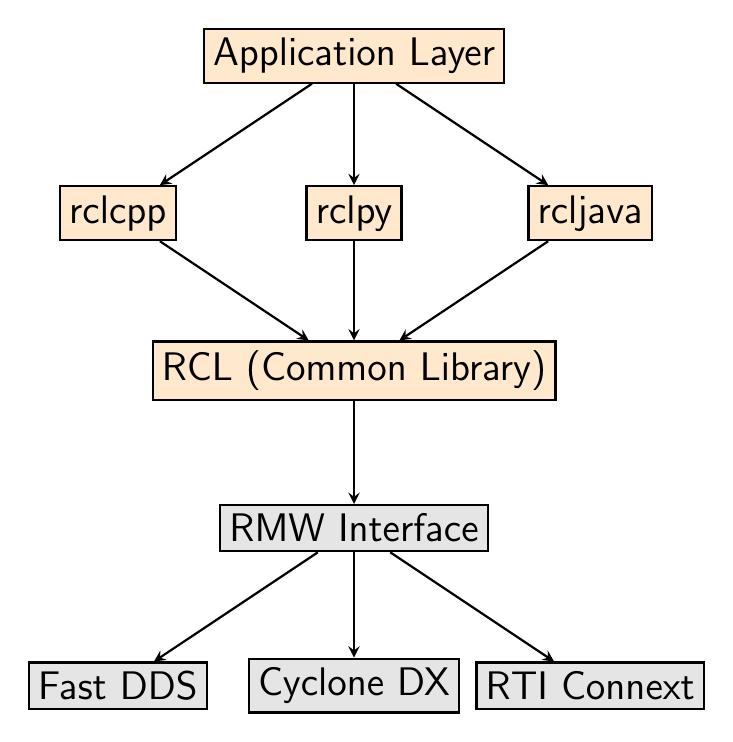
\begin{tikzpicture}[
    node distance=2cm,
    auto,
    thick,
    main node/.style={circle,fill=ros2blue!20,draw,font=\sffamily\Large\bfseries},
    lib node/.style={rectangle,fill=ros2orange!20,draw,font=\sffamily\Large},
    middleware node/.style={rectangle,fill=gray!20,draw,font=\sffamily\Large},
    arrow/.style={->,>=stealth,thick}
]

% Application Layer
\node[lib node] (app) at (0,6) {Application Layer};

% Client Libraries
\node[lib node] (rclcpp) at (-3,4) {rclcpp};
\node[lib node] (rclpy) at (0,4) {rclpy};
\node[lib node] (rcljava) at (3,4) {rcljava};

% RCL Layer
\node[lib node] (rcl) at (0,2) {RCL (Common Library)};

% RMW Layer
\node[middleware node] (rmw) at (0,0) {RMW Interface};

% DDS Implementations
\node[middleware node] (fastdds) at (-3,-2) {Fast DDS};
\node[middleware node] (cyclonedx) at (0,-2) {Cyclone DX};
\node[middleware node] (connext) at (3,-2) {RTI Connext};

% Arrows
\draw[arrow] (app) -- (rclcpp);
\draw[arrow] (app) -- (rclpy);
\draw[arrow] (app) -- (rcljava);
\draw[arrow] (rclcpp) -- (rcl);
\draw[arrow] (rclpy) -- (rcl);
\draw[arrow] (rcljava) -- (rcl);
\draw[arrow] (rcl) -- (rmw);
\draw[arrow] (rmw) -- (fastdds);
\draw[arrow] (rmw) -- (cyclonedx);
\draw[arrow] (rmw) -- (connext);

\end{tikzpicture}
\caption{ROS 2 Architecture Layers}
\label{fig:ros2_architecture}
\end{figure}

\section{Core Concepts}

\subsection{Nodes}
A \important{node} is a fundamental building block of ROS 2. It represents a single, modular purpose (e.g., controlling wheel motors, planning a path, etc.).

\begin{table}[H]
\centering
\begin{tabular}{|l|p{8cm}|}
\hline
\textbf{Property} & \textbf{Description} \\
\hline
Name & Unique identifier within the ROS graph \\
\hline
Namespace & Hierarchical organization of nodes \\
\hline
Publishers & Send data on specific topics \\
\hline
Subscribers & Receive data from specific topics \\
\hline
Services & Provide request-response functionality \\
\hline
Actions & Handle long-running tasks with feedback \\
\hline
Parameters & Runtime configuration values \\
\hline
\end{tabular}
\caption{Node Properties}
\label{tab:node_properties}
\end{table}

\subsection{Topics}
\important{Topics} are named buses over which nodes exchange messages. They implement a publish-subscribe pattern.

\begin{figure}[H]
\centering
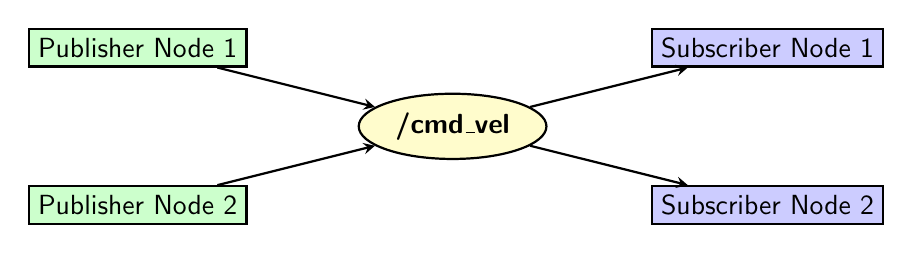
\begin{tikzpicture}[
    node distance=3cm,
    auto,
    thick,
    pub node/.style={rectangle,fill=green!20,draw,font=\sffamily},
    sub node/.style={rectangle,fill=blue!20,draw,font=\sffamily},
    topic node/.style={ellipse,fill=yellow!20,draw,font=\sffamily\bfseries},
    arrow/.style={->,>=stealth,thick}
]

\node[pub node] (pub1) at (-4,2) {Publisher Node 1};
\node[pub node] (pub2) at (-4,0) {Publisher Node 2};
\node[topic node] (topic) at (0,1) {/cmd\_vel};
\node[sub node] (sub1) at (4,2) {Subscriber Node 1};
\node[sub node] (sub2) at (4,0) {Subscriber Node 2};

\draw[arrow] (pub1) -- (topic);
\draw[arrow] (pub2) -- (topic);
\draw[arrow] (topic) -- (sub1);
\draw[arrow] (topic) -- (sub2);

\end{tikzpicture}
\caption{Topic Communication Pattern}
\label{fig:topic_pattern}
\end{figure}

\subsection{Services}
\important{Services} provide synchronous request-response communication between nodes.

\subsection{Actions}
\important{Actions} are used for long-running tasks that need feedback and can be preempted.

\chapter{Client Libraries}

\section{rclcpp (C++ Client Library)}

\subsection{Overview}
\code{rclcpp} is the C++ client library for ROS 2, providing object-oriented APIs for creating nodes, publishers, subscribers, services, and actions.

\subsection{Core Classes}

\begin{longtable}{|p{3cm}|p{4cm}|p{7cm}|}
\hline
\textbf{Class} & \textbf{Purpose} & \textbf{Key Methods} \\
\hline
\endhead
\code{rclcpp::Node} & Base class for ROS 2 nodes & \code{create\_publisher()}, \code{create\_subscription()}, \code{create\_service()}, \code{create\_client()} \\
\hline
\code{rclcpp::Publisher} & Publishes messages to topics & \code{publish()}, \code{get\_subscription\_count()} \\
\hline
\code{rclcpp::Subscription} & Receives messages from topics & Callback function, \code{get\_publisher\_count()} \\
\hline
\code{rclcpp::Service} & Provides service functionality & Callback function \\
\hline
\code{rclcpp::Client} & Calls services & \code{async\_send\_request()}, \code{wait\_for\_service()} \\
\hline
\code{rclcpp::Timer} & Periodic execution & \code{cancel()}, \code{reset()} \\
\hline
\code{rclcpp::Executor} & Manages node execution & \code{spin()}, \code{spin\_once()}, \code{add\_node()} \\
\hline
\caption{Core rclcpp Classes}
\label{tab:rclcpp_classes}
\end{longtable}

\subsection{Example: Simple Publisher}

\begin{lstlisting}[language=CPP, caption=Simple Publisher in C++]
#include <chrono>
#include <memory>
#include "rclcpp/rclcpp.hpp"
#include "std_msgs/msg/string.hpp"

using namespace std::chrono_literals;

class MinimalPublisher : public rclcpp::Node
{
public:
  MinimalPublisher() : Node("minimal_publisher"), count_(0)
  {
    publisher_ = this->create_publisher<std_msgs::msg::String>(
        "topic", 10);
    timer_ = this->create_wall_timer(
        500ms, std::bind(&MinimalPublisher::timer_callback, this));
  }

private:
  void timer_callback()
  {
    auto message = std_msgs::msg::String();
    message.data = "Hello, world! " + std::to_string(count_++);
    RCLCPP_INFO(this->get_logger(), "Publishing: '%s'", 
                message.data.c_str());
    publisher_->publish(message);
  }
  
  rclcpp::TimerBase::SharedPtr timer_;
  rclcpp::Publisher<std_msgs::msg::String>::SharedPtr publisher_;
  size_t count_;
};

int main(int argc, char * argv[])
{
  rclcpp::init(argc, argv);
  rclcpp::spin(std::make_shared<MinimalPublisher>());
  rclcpp::shutdown();
  return 0;
}
\end{lstlisting}

\subsubsection{Expected Output}
\begin{verbatim}
[INFO] [1234567890.123456789] [minimal_publisher]: Publishing: 'Hello, world! 0'
[INFO] [1234567890.623456789] [minimal_publisher]: Publishing: 'Hello, world! 1'
[INFO] [1234567891.123456789] [minimal_publisher]: Publishing: 'Hello, world! 2'
[INFO] [1234567891.623456789] [minimal_publisher]: Publishing: 'Hello, world! 3'
...
\end{verbatim}

\subsection{Example: Simple Subscriber}

\begin{lstlisting}[language=CPP, caption=Simple Subscriber in C++]
#include <memory>
#include "rclcpp/rclcpp.hpp"
#include "std_msgs/msg/string.hpp"

class MinimalSubscriber : public rclcpp::Node
{
public:
  MinimalSubscriber() : Node("minimal_subscriber")
  {
    subscription_ = this->create_subscription<std_msgs::msg::String>(
      "topic", 10, 
      std::bind(&MinimalSubscriber::topic_callback, this, 
                std::placeholders::_1));
  }

private:
  void topic_callback(const std_msgs::msg::String::SharedPtr msg) const
  {
    RCLCPP_INFO(this->get_logger(), "I heard: '%s'", msg->data.c_str());
  }
  
  rclcpp::Subscription<std_msgs::msg::String>::SharedPtr subscription_;
};

int main(int argc, char * argv[])
{
  rclcpp::init(argc, argv);
  rclcpp::spin(std::make_shared<MinimalSubscriber>());
  rclcpp::shutdown();
  return 0;
}
\end{lstlisting}

\subsubsection{Expected Output}
\begin{verbatim}
[INFO] [1234567890.123456789] [minimal_subscriber]: I heard: 'Hello, world! 0'
[INFO] [1234567890.623456789] [minimal_subscriber]: I heard: 'Hello, world! 1'
[INFO] [1234567891.123456789] [minimal_subscriber]: I heard: 'Hello, world! 2'
[INFO] [1234567891.623456789] [minimal_subscriber]: I heard: 'Hello, world! 3'
...
\end{verbatim}

\section{rclpy (Python Client Library)}

\subsection{Overview}
\code{rclpy} is the Python client library for ROS 2, providing Pythonic APIs for ROS 2 functionality.

\subsection{Core Classes}

\begin{longtable}{|p{3cm}|p{4cm}|p{7cm}|}
\hline
\textbf{Class} & \textbf{Purpose} & \textbf{Key Methods} \\
\hline
\endhead
\code{rclpy.node.Node} & Base class for ROS 2 nodes & \code{create\_publisher()}, \code{create\_subscription()}, \code{create\_service()}, \code{create\_client()} \\
\hline
\code{rclpy.publisher.Publisher} & Publishes messages to topics & \code{publish()}, \code{get\_subscription\_count()} \\
\hline
\code{rclpy.subscription.Subscription} & Receives messages from topics & Callback function \\
\hline
\code{rclpy.service.Service} & Provides service functionality & Callback function \\
\hline
\code{rclpy.client.Client} & Calls services & \code{call\_async()}, \code{wait\_for\_service()} \\
\hline
\code{rclpy.timer.Timer} & Periodic execution & \code{cancel()}, \code{reset()} \\
\hline
\caption{Core rclpy Classes}
\label{tab:rclpy_classes}
\end{longtable}

\subsection{Example: Simple Publisher}

\begin{lstlisting}[language=Python, caption=Simple Publisher in Python]
import rclpy
from rclpy.node import Node
from std_msgs.msg import String


class MinimalPublisher(Node):

    def __init__(self):
        super().__init__('minimal_publisher')
        self.publisher_ = self.create_publisher(String, 'topic', 10)
        timer_period = 0.5  # seconds
        self.timer = self.create_timer(timer_period, self.timer_callback)
        self.i = 0

    def timer_callback(self):
        msg = String()
        msg.data = f'Hello World: {self.i}'
        self.publisher_.publish(msg)
        self.get_logger().info(f'Publishing: "{msg.data}"')
        self.i += 1


def main(args=None):
    rclpy.init(args=args)
    
    minimal_publisher = MinimalPublisher()
    
    rclpy.spin(minimal_publisher)
    
    # Destroy the node explicitly
    minimal_publisher.destroy_node()
    rclpy.shutdown()


if __name__ == '__main__':
    main()
\end{lstlisting}

\subsubsection{Expected Output}
\begin{verbatim}
[INFO] [1234567890.123456789] [minimal_publisher]: Publishing: "Hello World: 0"
[INFO] [1234567890.623456789] [minimal_publisher]: Publishing: "Hello World: 1"
[INFO] [1234567891.123456789] [minimal_publisher]: Publishing: "Hello World: 2"
[INFO] [1234567891.623456789] [minimal_publisher]: Publishing: "Hello World: 3"
...
\end{verbatim}

\subsection{Example: Simple Subscriber}

\begin{lstlisting}[language=Python, caption=Simple Subscriber in Python]
import rclpy
from rclpy.node import Node
from std_msgs.msg import String


class MinimalSubscriber(Node):

    def __init__(self):
        super().__init__('minimal_subscriber')
        self.subscription = self.create_subscription(
            String,
            'topic',
            self.listener_callback,
            10)
        self.subscription  # prevent unused variable warning

    def listener_callback(self, msg):
        self.get_logger().info(f'I heard: "{msg.data}"')


def main(args=None):
    rclpy.init(args=args)
    
    minimal_subscriber = MinimalSubscriber()
    
    rclpy.spin(minimal_subscriber)
    
    # Destroy the node explicitly
    minimal_subscriber.destroy_node()
    rclpy.shutdown()


if __name__ == '__main__':
    main()
\end{lstlisting}

\subsubsection{Expected Output}
\begin{verbatim}
[INFO] [1234567890.123456789] [minimal_subscriber]: I heard: "Hello World: 0"
[INFO] [1234567890.623456789] [minimal_subscriber]: I heard: "Hello World: 1"
[INFO] [1234567891.123456789] [minimal_subscriber]: I heard: "Hello World: 2"
[INFO] [1234567891.623456789] [minimal_subscriber]: I heard: "Hello World: 3"
...
\end{verbatim}

\chapter{Messaging and Communication}

\section{Message Types}

ROS 2 uses strongly-typed messages for communication. Standard message types are defined in the \code{std\_msgs}, \code{geometry\_msgs}, \code{sensor\_msgs}, and other packages.

\subsection{Standard Message Types}

\begin{table}[H]
\centering
\begin{tabular}{|l|l|p{6cm}|}
\hline
\textbf{Package} & \textbf{Message Type} & \textbf{Description} \\
\hline
\code{std\_msgs} & \code{String} & Simple string message \\
\hline
\code{std\_msgs} & \code{Int32} & 32-bit integer \\
\hline
\code{std\_msgs} & \code{Float64} & 64-bit floating point \\
\hline
\code{geometry\_msgs} & \code{Twist} & Linear and angular velocity \\
\hline
\code{geometry\_msgs} & \code{Pose} & Position and orientation \\
\hline
\code{sensor\_msgs} & \code{Image} & Camera image data \\
\hline
\code{sensor\_msgs} & \code{LaserScan} & Laser range finder data \\
\hline
\end{tabular}
\caption{Common ROS 2 Message Types}
\label{tab:message_types}
\end{table}

\section{Services}

Services provide synchronous request-response communication between nodes.

\subsection{Example: Service Server (C++)}

\begin{lstlisting}[language=CPP, caption=Service Server in C++]
#include "rclcpp/rclcpp.hpp"
#include "example_interfaces/srv/add_two_ints.hpp"
#include <memory>

void add(const std::shared_ptr<example_interfaces::srv::AddTwoInts::Request> request,
         std::shared_ptr<example_interfaces::srv::AddTwoInts::Response> response)
{
  response->sum = request->a + request->b;
  RCLCPP_INFO(rclcpp::get_logger("rclcpp"), 
              "Incoming request\na: %ld b: %ld", request->a, request->b);
  RCLCPP_INFO(rclcpp::get_logger("rclcpp"), "sending back response: [%ld]", 
              response->sum);
}

int main(int argc, char **argv)
{
  rclcpp::init(argc, argv);

  std::shared_ptr<rclcpp::Node> node = 
      rclcpp::Node::make_shared("add_two_ints_server");

  rclcpp::Service<example_interfaces::srv::AddTwoInts>::SharedPtr service =
    node->create_service<example_interfaces::srv::AddTwoInts>(
        "add_two_ints", &add);

  RCLCPP_INFO(rclcpp::get_logger("rclcpp"), "Ready to add two ints.");

  rclcpp::spin(node);
  rclcpp::shutdown();
}
\end{lstlisting}

\subsection{Example: Service Client (C++)}

\begin{lstlisting}[language=CPP, caption=Service Client in C++]
#include "rclcpp/rclcpp.hpp"
#include "example_interfaces/srv/add_two_ints.hpp"
#include <chrono>
#include <cstdlib>
#include <memory>

using namespace std::chrono_literals;

int main(int argc, char **argv)
{
  rclcpp::init(argc, argv);

  if (argc != 3) {
      RCLCPP_INFO(rclcpp::get_logger("rclcpp"), 
                  "usage: add_two_ints_client X Y");
      return 1;
  }

  std::shared_ptr<rclcpp::Node> node = 
      rclcpp::Node::make_shared("add_two_ints_client");
  rclcpp::Client<example_interfaces::srv::AddTwoInts>::SharedPtr client =
    node->create_client<example_interfaces::srv::AddTwoInts>("add_two_ints");

  auto request = std::make_shared<example_interfaces::srv::AddTwoInts::Request>();
  request->a = atoll(argv[1]);
  request->b = atoll(argv[2]);

  while (!client->wait_for_service(1s)) {
    if (!rclcpp::ok()) {
      RCLCPP_ERROR(rclcpp::get_logger("rclcpp"), 
                   "Interrupted while waiting for the service. Exiting.");
      return 0;
    }
    RCLCPP_INFO(rclcpp::get_logger("rclcpp"), 
                "service not available, waiting again...");
  }

  auto result = client->async_send_request(request);
  // Wait for the result.
  if (rclcpp::spin_until_future_complete(node, result) ==
    rclcpp::FutureReturnCode::SUCCESS)
  {
    RCLCPP_INFO(rclcpp::get_logger("rclcpp"), "Sum: %ld", result.get()->sum);
  } else {
    RCLCPP_ERROR(rclcpp::get_logger("rclcpp"), "Failed to call service add_two_ints");
  }

  rclcpp::shutdown();
  return 0;
}
\end{lstlisting}

\subsubsection{Expected Output}
\textbf{Server:}
\begin{verbatim}
[INFO] [1234567890.123456789] [rclcpp]: Ready to add two ints.
[INFO] [1234567890.223456789] [rclcpp]: Incoming request
a: 2 b: 3
[INFO] [1234567890.223456789] [rclcpp]: sending back response: [5]
\end{verbatim}

\textbf{Client:}
\begin{verbatim}
[INFO] [1234567890.223456789] [rclcpp]: Sum: 5
\end{verbatim}

\chapter{Actions}

Actions are used for long-running tasks that provide feedback and can be preempted.

\section{Action Structure}

Actions consist of three parts:
\begin{itemize}
\item \important{Goal}: What we want to achieve
\item \important{Feedback}: Progress updates during execution
\item \important{Result}: Final outcome of the action
\end{itemize}

\begin{figure}[H]
\centering
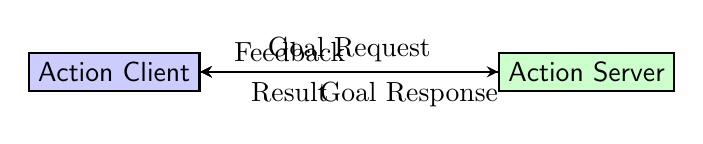
\begin{tikzpicture}[
    node distance=2cm,
    auto,
    thick,
    client node/.style={rectangle,fill=blue!20,draw,font=\sffamily},
    server node/.style={rectangle,fill=green!20,draw,font=\sffamily},
    arrow/.style={->,>=stealth,thick}
]

\node[client node] (client) at (0,0) {Action Client};
\node[server node] (server) at (6,0) {Action Server};

\draw[arrow] (client) -- node[above] {Goal Request} (server);
\draw[arrow] (server) -- node[below, pos=0.3] {Goal Response} (client);
\draw[arrow] (server) -- node[above, pos=0.7] {Feedback} (client);
\draw[arrow] (server) -- node[below, pos=0.7] {Result} (client);

\end{tikzpicture}
\caption{Action Communication Pattern}
\label{fig:action_pattern}
\end{figure}

\section{Example: Fibonacci Action Server (Python)}

\begin{lstlisting}[language=Python, caption=Fibonacci Action Server in Python]
import rclpy
from rclpy.action import ActionServer
from rclpy.node import Node
from action_tutorials_interfaces.action import Fibonacci


class FibonacciActionServer(Node):

    def __init__(self):
        super().__init__('fibonacci_action_server')
        self._action_server = ActionServer(
            self,
            Fibonacci,
            'fibonacci',
            self.execute_callback)

    def execute_callback(self, goal_handle):
        self.get_logger().info('Executing goal...')

        feedback_msg = Fibonacci.Feedback()
        feedback_msg.partial_sequence = [0, 1]

        for i in range(1, goal_handle.request.order):
            feedback_msg.partial_sequence.append(
                feedback_msg.partial_sequence[i] + 
                feedback_msg.partial_sequence[i-1])
            self.get_logger().info(
                f'Feedback: {feedback_msg.partial_sequence}')
            goal_handle.publish_feedback(feedback_msg)
            
            if goal_handle.is_cancel_requested:
                goal_handle.canceled()
                self.get_logger().info('Goal canceled')
                return Fibonacci.Result()

        goal_handle.succeed()

        result = Fibonacci.Result()
        result.sequence = feedback_msg.partial_sequence
        return result


def main(args=None):
    rclpy.init(args=args)

    fibonacci_action_server = FibonacciActionServer()

    rclpy.spin(fibonacci_action_server)


if __name__ == '__main__':
    main()
\end{lstlisting}

\chapter{Quality of Service (QoS)}

Quality of Service (QoS) policies allow you to configure the behavior of publishers and subscribers.

\section{QoS Policies}

\begin{table}[H]
\centering
\begin{tabular}{|l|p{3cm}|p{7cm}|}
\hline
\textbf{Policy} & \textbf{Options} & \textbf{Description} \\
\hline
Reliability & RELIABLE, BEST\_EFFORT & Whether messages are guaranteed to arrive \\
\hline
Durability & VOLATILE, TRANSIENT\_LOCAL & Whether messages are stored for late-joining subscribers \\
\hline
History & KEEP\_LAST, KEEP\_ALL & How many messages to keep in the queue \\
\hline
Depth & Integer & Number of messages to keep (when KEEP\_LAST) \\
\hline
Deadline & Duration & Maximum time between messages \\
\hline
Lifespan & Duration & How long messages remain valid \\
\hline
Liveliness & AUTOMATIC, MANUAL\_BY\_TOPIC & How to determine if publishers are alive \\
\hline
\end{tabular}
\caption{QoS Policies}
\label{tab:qos_policies}
\end{table}

\section{Example: Custom QoS (C++)}

\begin{lstlisting}[language=CPP, caption=Custom QoS Settings in C++]
#include "rclcpp/rclcpp.hpp"
#include "std_msgs/msg/string.hpp"

class CustomQoSPublisher : public rclcpp::Node
{
public:
  CustomQoSPublisher() : Node("custom_qos_publisher")
  {
    // Create custom QoS profile
    auto qos = rclcpp::QoS(10)  // Keep last 10 messages
                  .reliability(rclcpp::ReliabilityPolicy::Reliable)
                  .durability(rclcpp::DurabilityPolicy::TransientLocal)
                  .deadline(std::chrono::seconds(2))
                  .lifespan(std::chrono::seconds(5));

    publisher_ = this->create_publisher<std_msgs::msg::String>(
        "topic", qos);
        
    timer_ = this->create_wall_timer(
        std::chrono::milliseconds(1000),
        std::bind(&CustomQoSPublisher::timer_callback, this));
  }

private:
  void timer_callback()
  {
    auto message = std_msgs::msg::String();
    message.data = "Hello with custom QoS!";
    publisher_->publish(message);
  }
  
  rclcpp::Publisher<std_msgs::msg::String>::SharedPtr publisher_;
  rclcpp::TimerBase::SharedPtr timer_;
};
\end{lstlisting}

\chapter{Parameters}

Parameters provide a way to configure nodes at runtime.

\section{Parameter Types}

ROS 2 supports the following parameter types:
\begin{itemize}
\item \code{bool}
\item \code{int64}
\item \code{double}
\item \code{string}
\item \code{byte\_array}
\item \code{bool\_array}
\item \code{int64\_array}
\item \code{double\_array}
\item \code{string\_array}
\end{itemize}

\section{Example: Parameter Node (Python)}

\begin{lstlisting}[language=Python, caption=Parameter Usage in Python]
import rclpy
from rclpy.node import Node
from rcl_interfaces.msg import ParameterDescriptor


class ParameterNode(Node):

    def __init__(self):
        super().__init__('parameter_node')
        
        # Declare parameters with descriptions
        my_parameter_descriptor = ParameterDescriptor(
            description='This parameter controls the timer period.')
        
        self.declare_parameter('my_parameter', 'world', my_parameter_descriptor)
        self.declare_parameter('timer_period', 1.0)
        
        # Create timer that uses parameter
        timer_period = self.get_parameter('timer_period').get_parameter_value().double_value
        self.timer = self.create_timer(timer_period, self.timer_callback)

    def timer_callback(self):
        my_param = self.get_parameter('my_parameter').get_parameter_value().string_value
        self.get_logger().info(f'Hello {my_param}!')
        
        # You can also get all parameters
        all_params = self.get_parameters(['my_parameter', 'timer_period'])
        for param in all_params:
            self.get_logger().info(f'{param.name}: {param.value}')


def main(args=None):
    rclpy.init(args=args)
    node = ParameterNode()
    rclpy.spin(node)
    rclpy.shutdown()


if __name__ == '__main__':
    main()
\end{lstlisting}

\chapter{Launch Files}

Launch files provide a way to start multiple nodes and configure the system.

\section{Python Launch Files}

\begin{lstlisting}[language=Python, caption=Python Launch File Example]
from launch import LaunchDescription
from launch_ros.actions import Node
from launch.actions import DeclareLaunchArgument
from launch.substitutions import LaunchConfiguration


def generate_launch_description():
    # Declare launch arguments
    namespace_arg = DeclareLaunchArgument(
        'namespace',
        default_value='my_robot',
        description='Namespace for the nodes'
    )
    
    use_sim_time_arg = DeclareLaunchArgument(
        'use_sim_time',
        default_value='false',
        description='Use simulation time'
    )

    # Launch nodes
    talker_node = Node(
        package='demo_nodes_cpp',
        executable='talker',
        name='talker',
        namespace=LaunchConfiguration('namespace'),
        parameters=[{
            'use_sim_time': LaunchConfiguration('use_sim_time')
        }],
        remappings=[
            ('chatter', 'my_topic')
        ]
    )

    listener_node = Node(
        package='demo_nodes_py',
        executable='listener',
        name='listener',
        namespace=LaunchConfiguration('namespace'),
        parameters=[{
            'use_sim_time': LaunchConfiguration('use_sim_time')
        }],
        remappings=[
            ('chatter', 'my_topic')
        ]
    )

    return LaunchDescription([
        namespace_arg,
        use_sim_time_arg,
        talker_node,
        listener_node
    ])
\end{lstlisting}

\chapter{Package Structure and Build System}

\section{Package Structure}

A typical ROS 2 package has the following structure:

\begin{lstlisting}[caption=Package Structure]
my_package/
|-- CMakeLists.txt          (for C++ packages)
|-- setup.py               (for Python packages)
|-- setup.cfg              (for Python packages)
|-- package.xml
|-- src/
|   +-- my_package/        (Python source code)
|-- include/
|   +-- my_package/        (C++ headers)
|-- launch/
|   +-- my_launch.py
|-- config/
|   +-- params.yaml
|-- msg/
|   +-- MyMessage.msg
|-- srv/
|   +-- MyService.srv
|-- action/
|   +-- MyAction.action
+-- README.md
\end{lstlisting}

\section{package.xml}

\begin{lstlisting}[language=XML, caption=Example package.xml]
<?xml version="1.0"?>
<?xml-model href="http://download.ros.org/schema/package_format3.xsd" 
            schematypens="http://www.w3.org/2001/XMLSchema"?>
<package format="3">
  <name>my_package</name>
  <version>0.0.1</version>
  <description>Example ROS 2 package</description>
  <maintainer email="user@example.com">User Name</maintainer>
  <license>Apache-2.0</license>

  <buildtool_depend>ament_cmake</buildtool_depend>
  
  <depend>rclcpp</depend>
  <depend>std_msgs</depend>
  <depend>geometry_msgs</depend>
  
  <test_depend>ament_lint_auto</test_depend>
  <test_depend>ament_lint_common</test_depend>

  <export>
    <build_type>ament_cmake</build_type>
  </export>
</package>
\end{lstlisting}

\chapter{Advanced Topics}

\section{Custom Message Types}

\subsection{Defining Custom Messages}

\begin{lstlisting}[caption=Custom Message Definition (PersonMessage.msg)]
string first_name
string last_name
uint8 age
float64 height
bool is_student
\end{lstlisting}

\subsection{Using Custom Messages (C++)}

\begin{lstlisting}[language=CPP, caption=Using Custom Messages in C++]
#include "rclcpp/rclcpp.hpp"
#include "my_package/msg/person_message.hpp"

class PersonPublisher : public rclcpp::Node
{
public:
  PersonPublisher() : Node("person_publisher")
  {
    publisher_ = this->create_publisher<my_package::msg::PersonMessage>(
        "person_info", 10);
    timer_ = this->create_wall_timer(
        std::chrono::seconds(1),
        std::bind(&PersonPublisher::timer_callback, this));
  }

private:
  void timer_callback()
  {
    auto message = my_package::msg::PersonMessage();
    message.first_name = "John";
    message.last_name = "Doe";
    message.age = 30;
    message.height = 1.75;
    message.is_student = false;
    
    RCLCPP_INFO(this->get_logger(), "Publishing person info");
    publisher_->publish(message);
  }
  
  rclcpp::Publisher<my_package::msg::PersonMessage>::SharedPtr publisher_;
  rclcpp::TimerBase::SharedPtr timer_;
};
\end{lstlisting}

\section{Node Composition}

Node composition allows multiple nodes to run in the same process for better performance.

\begin{lstlisting}[language=CPP, caption=Composable Node Example]
#include "rclcpp/rclcpp.hpp"
#include "rclcpp_components/register_node_macro.hpp"
#include "std_msgs/msg/string.hpp"

namespace composition
{

class Talker : public rclcpp::Node
{
public:
  explicit Talker(const rclcpp::NodeOptions & options)
  : Node("talker", options)
  {
    pub_ = create_publisher<std_msgs::msg::String>("chatter", 10);
    timer_ = create_wall_timer(
        std::chrono::milliseconds(1000),
        std::bind(&Talker::on_timer, this));
  }

private:
  void on_timer()
  {
    auto msg = std::make_unique<std_msgs::msg::String>();
    msg->data = "Hello World: " + std::to_string(count_++);
    RCLCPP_INFO(this->get_logger(), "Publishing: '%s'", msg->data.c_str());
    pub_->publish(std::move(msg));
  }

  rclcpp::Publisher<std_msgs::msg::String>::SharedPtr pub_;
  rclcpp::TimerBase::SharedPtr timer_;
  size_t count_ = 0;
};

}  // namespace composition

RCLCPP_COMPONENTS_REGISTER_NODE(composition::Talker)
\end{lstlisting}

\chapter{Tools and Utilities}

\section{Command-Line Tools}

ROS 2 provides many command-line tools for debugging and introspection:

\begin{table}[H]
\centering
\begin{tabular}{|l|p{8cm}|}
\hline
\textbf{Command} & \textbf{Description} \\
\hline
\code{ros2 node list} & List running nodes \\
\hline
\code{ros2 topic list} & List active topics \\
\hline
\code{ros2 topic echo /topic\_name} & Display messages on a topic \\
\hline
\code{ros2 topic pub /topic\_name msg\_type data} & Publish to a topic \\
\hline
\code{ros2 service list} & List available services \\
\hline
\code{ros2 service call /service\_name srv\_type request} & Call a service \\
\hline
\code{ros2 param list} & List parameters \\
\hline
\code{ros2 param get /node\_name param\_name} & Get parameter value \\
\hline
\code{ros2 param set /node\_name param\_name value} & Set parameter value \\
\hline
\code{ros2 launch package\_name launch\_file.py} & Run launch file \\
\hline
\code{ros2 bag record /topic\_name} & Record topic data \\
\hline
\code{ros2 bag play bag\_file} & Replay recorded data \\
\hline
\end{tabular}
\caption{Common ROS 2 Commands}
\label{tab:ros2_commands}
\end{table}

\section{rqt Tools}

\code{rqt} provides graphical tools for ROS 2:

\begin{itemize}
\item \code{rqt\_graph}: Visualize the node graph
\item \code{rqt\_plot}: Plot numeric data from topics
\item \code{rqt\_console}: View log messages
\item \code{rqt\_param}: Edit parameters graphically
\item \code{rqt\_service\_caller}: Call services through GUI
\item \code{rqt\_topic}: Monitor topics
\end{itemize}

\chapter{Best Practices and Design Patterns}

\section{Node Design Principles}

\begin{enumerate}
\item \important{Single Responsibility}: Each node should have one clear purpose
\item \important{Loose Coupling}: Minimize dependencies between nodes
\item \important{Interface Segregation}: Use specific message types rather than generic ones
\item \important{Composition over Inheritance}: Prefer composition for complex behaviors
\item \important{Error Handling}: Always handle errors gracefully
\end{enumerate}

\section{Performance Considerations}

\subsection{Message Size}
\begin{itemize}
\item Keep messages as small as possible
\item Use appropriate data types (don't use \code{double} when \code{float} suffices)
\item Consider compression for large data
\end{itemize}

\subsection{Publishing Frequency}
\begin{itemize}
\item Match publishing frequency to actual needs
\item Use timers for periodic publishing
\item Consider QoS settings for reliability vs. performance trade-offs
\end{itemize}

\subsection{Memory Management}
\begin{itemize}
\item Use smart pointers in C++
\item Avoid memory leaks in long-running nodes
\item Consider zero-copy transport for large messages
\end{itemize}

\chapter{Debugging and Testing}

\section{Logging}

ROS 2 provides structured logging with different severity levels:

\begin{lstlisting}[language=CPP, caption=Logging in C++]
RCLCPP_DEBUG(this->get_logger(), "Debug message");
RCLCPP_INFO(this->get_logger(), "Info message");
RCLCPP_WARN(this->get_logger(), "Warning message");
RCLCPP_ERROR(this->get_logger(), "Error message");
RCLCPP_FATAL(this->get_logger(), "Fatal message");
\end{lstlisting}

\begin{lstlisting}[language=Python, caption=Logging in Python]
self.get_logger().debug('Debug message')
self.get_logger().info('Info message')
self.get_logger().warn('Warning message')
self.get_logger().error('Error message')
self.get_logger().fatal('Fatal message')
\end{lstlisting}

\section{Unit Testing}

\subsection{C++ Testing with gtest}

\begin{lstlisting}[language=CPP, caption=Unit Test Example in C++]
#include <gtest/gtest.h>
#include "rclcpp/rclcpp.hpp"
#include "my_package/my_node.hpp"

class TestMyNode : public ::testing::Test
{
protected:
  void SetUp() override
  {
    rclcpp::init(0, nullptr);
    node_ = std::make_shared<MyNode>();
  }

  void TearDown() override
  {
    rclcpp::shutdown();
  }

  std::shared_ptr<MyNode> node_;
};

TEST_F(TestMyNode, TestCalculation)
{
  int result = node_->calculate(2, 3);
  EXPECT_EQ(result, 5);
}

int main(int argc, char **argv)
{
  ::testing::InitGoogleTest(&argc, argv);
  return RUN_ALL_TESTS();
}
\end{lstlisting}

\subsection{Python Testing with pytest}

\begin{lstlisting}[language=Python, caption=Unit Test Example in Python]
import pytest
import rclpy
from my_package.my_node import MyNode


class TestMyNode:

    @classmethod
    def setup_class(cls):
        rclpy.init()

    @classmethod
    def teardown_class(cls):
        rclpy.shutdown()

    def setup_method(self):
        self.node = MyNode()

    def teardown_method(self):
        self.node.destroy_node()

    def test_calculation(self):
        result = self.node.calculate(2, 3)
        assert result == 5

    def test_message_processing(self):
        # Test message processing logic
        processed = self.node.process_message("test")
        assert processed == "processed: test"
\end{lstlisting}

\chapter{Migration from ROS 1}

\section{Key Differences}

\begin{table}[H]
\centering
\begin{tabular}{|l|l|l|}
\hline
\textbf{Aspect} & \textbf{ROS 1} & \textbf{ROS 2} \\
\hline
Master & Required & Not required \\
\hline
Language Support & C++, Python & C++, Python, others \\
\hline
Real-time & Limited & Native support \\
\hline
Security & Basic & Advanced \\
\hline
Platform Support & Linux & Linux, Windows, macOS \\
\hline
Communication & TCP/UDP & DDS \\
\hline
Build System & catkin & ament \\
\hline
\end{tabular}
\caption{ROS 1 vs ROS 2 Comparison}
\label{tab:ros1_vs_ros2}
\end{table}

\section{Migration Checklist}

\begin{enumerate}
\item Update package.xml to format 3
\item Replace CMakeLists.txt with ament\_cmake
\item Update include statements and namespaces
\item Replace rospy/roscpp with rclpy/rclcpp
\item Update launch files to Python format
\item Test QoS settings for reliability
\item Update parameter handling
\item Verify timing behavior
\end{enumerate}

\chapter{Future Roadmap and Ecosystem}

\section{ROS 2 Roadmap}

The ROS 2 project continues to evolve with regular releases:

\begin{table}[H]
\centering
\begin{tabular}{|l|l|l|}
\hline
\textbf{Release} & \textbf{Date} & \textbf{Key Features} \\
\hline
Galactic & May 2021 & ROS 2 maturation \\
\hline
Humble & May 2022 & LTS Release \\
\hline
Iron & May 2023 & Improved performance \\
\hline
Jazzy & May 2024 & Enhanced security \\
\hline
\end{tabular}
\caption{Recent ROS 2 Releases}
\label{tab:ros2_releases}
\end{table}

\section{Ecosystem Packages}

Popular packages in the ROS 2 ecosystem:

\begin{itemize}
\item \important{Navigation2}: Mobile robot navigation
\item \important{MoveIt2}: Motion planning framework
\item \important{Gazebo}: 3D robot simulation
\item \important{RViz2}: 3D visualization tool
\item \important{tf2}: Coordinate frame transformations
\item \important{rosbag2}: Data recording and playback
\item \important{ros2\_control}: Real-time control framework
\item \important{micro-ROS}: ROS 2 for microcontrollers
\end{itemize}

\appendix

\chapter{Message Reference}

\section{geometry\_msgs}

\subsection{Twist Message}

\begin{lstlisting}[caption=geometry\_msgs/Twist.msg]
# This expresses velocity in free space broken into its linear and angular parts.
Vector3 linear
  float64 x
  float64 y
  float64 z
Vector3 angular
  float64 x
  float64 y
  float64 z
\end{lstlisting}

\subsection{Pose Message}

\begin{lstlisting}[caption=geometry\_msgs/Pose.msg]
# Position
Point position
  float64 x
  float64 y
  float64 z

# Orientation
Quaternion orientation
  float64 x
  float64 y
  float64 z
  float64 w
\end{lstlisting}

\chapter{Service Reference}

\section{example\_interfaces}

\subsection{AddTwoInts Service}

\begin{lstlisting}[caption=example\_interfaces/srv/AddTwoInts.srv]
int64 a
int64 b
---
int64 sum
\end{lstlisting}

\chapter{Build System Reference}

\section{CMakeLists.txt Template}

\begin{lstlisting}[caption=CMakeLists.txt for C++ package]
cmake_minimum_required(VERSION 3.8)
project(my_package)

if(CMAKE_COMPILER_IS_GNUCXX OR CMAKE_CXX_COMPILER_ID MATCHES "Clang")
  add_compile_options(-Wall -Wextra -Wpedantic)
endif()

# find dependencies
find_package(ament_cmake REQUIRED)
find_package(rclcpp REQUIRED)
find_package(std_msgs REQUIRED)

# Create executable
add_executable(my_node src/my_node.cpp)
ament_target_dependencies(my_node rclcpp std_msgs)

# Install
install(TARGETS
  my_node
  DESTINATION lib/${PROJECT_NAME})

if(BUILD_TESTING)
  find_package(ament_lint_auto REQUIRED)
  ament_lint_auto_find_test_dependencies()
endif()

ament_package()
\end{lstlisting}

\section{setup.py Template}

\begin{lstlisting}[language=Python, caption=setup.py for Python package]
from setuptools import setup

package_name = 'my_package'

setup(
    name=package_name,
    version='0.0.1',
    packages=[package_name],
    data_files=[
        ('share/ament_index/resource_index/packages',
            ['resource/' + package_name]),
        ('share/' + package_name, ['package.xml']),
        ('share/' + package_name + '/launch', ['launch/my_launch.py']),
        ('share/' + package_name + '/config', ['config/params.yaml']),
    ],
    install_requires=['setuptools'],
    zip_safe=True,
    maintainer='Your Name',
    maintainer_email='your.email@example.com',
    description='Package description',
    license='Apache License 2.0',
    tests_require=['pytest'],
    entry_points={
        'console_scripts': [
            'my_node = my_package.my_node:main',
        ],
    },
)
\end{lstlisting}

\backmatter

\chapter{Glossary}

\begin{description}
\item[Action] Long-running tasks with feedback and preemption capabilities
\item[Client Library] Language-specific API for ROS 2 functionality
\item[DDS] Data Distribution Service - middleware standard used by ROS 2
\item[Executor] Component that manages node execution and callback handling
\item[Launch File] Configuration file to start multiple nodes and set parameters
\item[Message] Data structure for communication between nodes
\item[Node] Fundamental building block of ROS 2 applications
\item[Parameter] Runtime configuration value for nodes
\item[Publisher] Sends messages to a topic
\item[QoS] Quality of Service - policies that control communication behavior
\item[Service] Synchronous request-response communication pattern
\item[Subscriber] Receives messages from a topic
\item[Topic] Named channel for asynchronous message passing
\item[Workspace] Directory containing ROS 2 packages
\end{description}

\chapter{Bibliography}

\begin{thebibliography}{9}

\bibitem{ros2docs}
Open Robotics. \textit{ROS 2 Documentation}. 
\url{https://docs.ros.org/en/humble/}

\bibitem{ros2design}
Dirk Thomas, et al. \textit{ROS 2 Design Documentation}. 
\url{https://design.ros2.org/}

\bibitem{ddsfoundation}
Object Management Group. \textit{Data Distribution Service (DDS) Specification}. 
\url{https://www.omg.org/spec/DDS/}

\bibitem{ros2tutorials}
Open Robotics. \textit{ROS 2 Tutorials}. 
\url{https://docs.ros.org/en/humble/Tutorials.html}

\bibitem{rclcpp}
Open Robotics. \textit{rclcpp Documentation}. 
\url{https://docs.ros2.org/humble/api/rclcpp/}

\bibitem{rclpy}
Open Robotics. \textit{rclpy Documentation}. 
\url{https://docs.ros2.org/humble/api/rclpy/}

\end{thebibliography}

% Index would be here if makeindex was used

\end{document}